\documentclass[sigconf, authordraft]{acmart}

\usepackage{booktabs} % For formal tables


% Copyright
%\setcopyright{none}
%\setcopyright{acmcopyright}
%\setcopyright{acmlicensed}
\setcopyright{rightsretained}
%\setcopyright{usgov}
%\setcopyright{usgovmixed}
%\setcopyright{cagov}
%\setcopyright{cagovmixed}


% DOI
\acmDOI{10.475/123_4}

% ISBN
\acmISBN{123-4567-24-567/08/06}

%Conference
\acmConference[WOODSTOCK'97]{ACM Woodstock conference}{July 1997}{El
  Paso, Texas USA} 
\acmYear{1997}
\copyrightyear{2016}

\acmPrice{15.00}

\acmSubmissionID{123-A12-B3}

\begin{document}
\title{SIG Proceedings Paper in LaTeX Format}
\titlenote{Produces the permission block, and
  copyright information}
\subtitle{Extended Abstract}
\subtitlenote{The full version of the author's guide is available as
  \texttt{acmart.pdf} document}


\author{Ben Trovato}
\authornote{Dr.~Trovato insisted his name be first.}
\orcid{1234-5678-9012}
\affiliation{%
  \institution{Institute for Clarity in Documentation}
  \streetaddress{P.O. Box 1212}
  \city{Dublin} 
  \state{Ohio} 
  \postcode{43017-6221}
}
\email{trovato@corporation.com}

\author{G.K.M. Tobin}
\authornote{The secretary disavows any knowledge of this author's actions.}
\affiliation{%
  \institution{Institute for Clarity in Documentation}
  \streetaddress{P.O. Box 1212}
  \city{Dublin} 
  \state{Ohio} 
  \postcode{43017-6221}
}
\email{webmaster@marysville-ohio.com}

\author{Lars Th{\o}rv{\"a}ld}
\authornote{This author is the
  one who did all the really hard work.}
\affiliation{%
  \institution{The Th{\o}rv{\"a}ld Group}
  \streetaddress{1 Th{\o}rv{\"a}ld Circle}
  \city{Hekla} 
  \country{Iceland}}
\email{larst@affiliation.org}

\author{Lawrence P. Leipuner}
\affiliation{
  \institution{Brookhaven Laboratories}
  \streetaddress{P.O. Box 5000}}
\email{lleipuner@researchlabs.org}

\author{Sean Fogarty}
\affiliation{%
  \institution{NASA Ames Research Center}
  \city{Moffett Field}
  \state{California} 
  \postcode{94035}}
\email{fogartys@amesres.org}

\author{Charles Palmer}
\affiliation{%
  \institution{Palmer Research Laboratories}
  \streetaddress{8600 Datapoint Drive}
  \city{San Antonio}
  \state{Texas} 
  \postcode{78229}}
\email{cpalmer@prl.com}

\author{John Smith}
\affiliation{\institution{The Th{\o}rv{\"a}ld Group}}
\email{jsmith@affiliation.org}

\author{Julius P.~Kumquat}
\affiliation{\institution{The Kumquat Consortium}}
\email{jpkumquat@consortium.net}

% The default list of authors is too long for headers.
\renewcommand{\shortauthors}{B. Trovato et al.}


\begin{abstract}
This paper provides a sample of a \LaTeX\ document which conforms,
somewhat loosely, to the formatting guidelines for
ACM SIG Proceedings.\footnote{This is an abstract footnote}
\end{abstract}

%
% The code below should be generated by the tool at
% http://dl.acm.org/ccs.cfm
% Please copy and paste the code instead of the example below. 
%
\begin{CCSXML}
<ccs2012>
 <concept>
  <concept_id>10010520.10010553.10010562</concept_id>
  <concept_desc>Computer systems organization~Embedded systems</concept_desc>
  <concept_significance>500</concept_significance>
 </concept>
 <concept>
  <concept_id>10010520.10010575.10010755</concept_id>
  <concept_desc>Computer systems organization~Redundancy</concept_desc>
  <concept_significance>300</concept_significance>
 </concept>
 <concept>
  <concept_id>10010520.10010553.10010554</concept_id>
  <concept_desc>Computer systems organization~Robotics</concept_desc>
  <concept_significance>100</concept_significance>
 </concept>
 <concept>
  <concept_id>10003033.10003083.10003095</concept_id>
  <concept_desc>Networks~Network reliability</concept_desc>
  <concept_significance>100</concept_significance>
 </concept>
</ccs2012>  
\end{CCSXML}

\ccsdesc[500]{Computer systems organization~Embedded systems}
\ccsdesc[300]{Computer systems organization~Redundancy}
\ccsdesc{Computer systems organization~Robotics}
\ccsdesc[100]{Networks~Network reliability}


\keywords{ACM proceedings, \LaTeX, text tagging}


\maketitle

\section{Introduction}

This means the model does not have to explicitly
store gigantic phrase tables and language models
as in  the case  of standard  MT; hence,  NMT has
a small memory footprint.   Lastly,  implementing
NMT decoders is easy unlike the highly intricate
decoders in standard MT.

\section{Neural Machine Translations}
NMT is an approach to machine translation that uses a large neural network. It departs from phrases-based statistical approaches that use separately engineerd subcomponents.Neural machine translation (NMT) is not a drastic step beyond what has been traditionally done in statistical machine translation (SMT). MNT starts emitting one target word a time  as illustrated in. NMT is often a large neural network that is trained in an end-to-end fashion and has the abil-ity to generalize well to very long word sequences.

\subsection{Encoder and decoder arquitecture}

A  neural  machine  translation  system  is  a  neural
network that directly models the conditional prob-ability $p(y|x)$ of translating a source sentence,$x_{1}$,...,$x_{n}$  to a target sentence $y_{1}$,...,$y_{n}$ A basic form of NMT consists of two components: $(a)$ an which computes a representations for each source sentence and $(b)$ a decoder which generates one target word at a time and hence decomposes the conditional
probability as:

% Introduce a new line

\begin{gather*}
  \log p(y|x) = \sum_{j=1}^{m}log p(y_{j}|y<j,s)
\end{gather*}

\begin{center}

\includegraphics[width=0.7\columnwidth]{nmt} \\% Example image
    Figura 1. Encoder-decoder architecture
\end{center}

\subsection{Long short term memory}
We consider as examples a deep multi-layer RNN which is unidirectional and uses LSTM as a recurrent unit. We show an example of such a model in Figure 2. In this example, we build a model to translate a source sentence "I am a student" into a target sentence "Je suis étudiant". At a high level, the NMT model consists of two recurrent neural networks: the encoder RNN simply consumes the input source words without making any prediction; the decoder, on the other hand, processes the target sentence while predicting the next words.


\begin{gather*}
  f_{t} = \sigma(W_{f}[h_{t-1},x_{t}]+b_{f}) \\
  i_{t} = \sigma(W_{i}[h_{t-1},x_{t}]+b_{i}) \\
  C_{t} = tanh(W_{c}[h_{t-1},x_{t}]+b_{c})   \\
\end{gather*}


\begin{center}
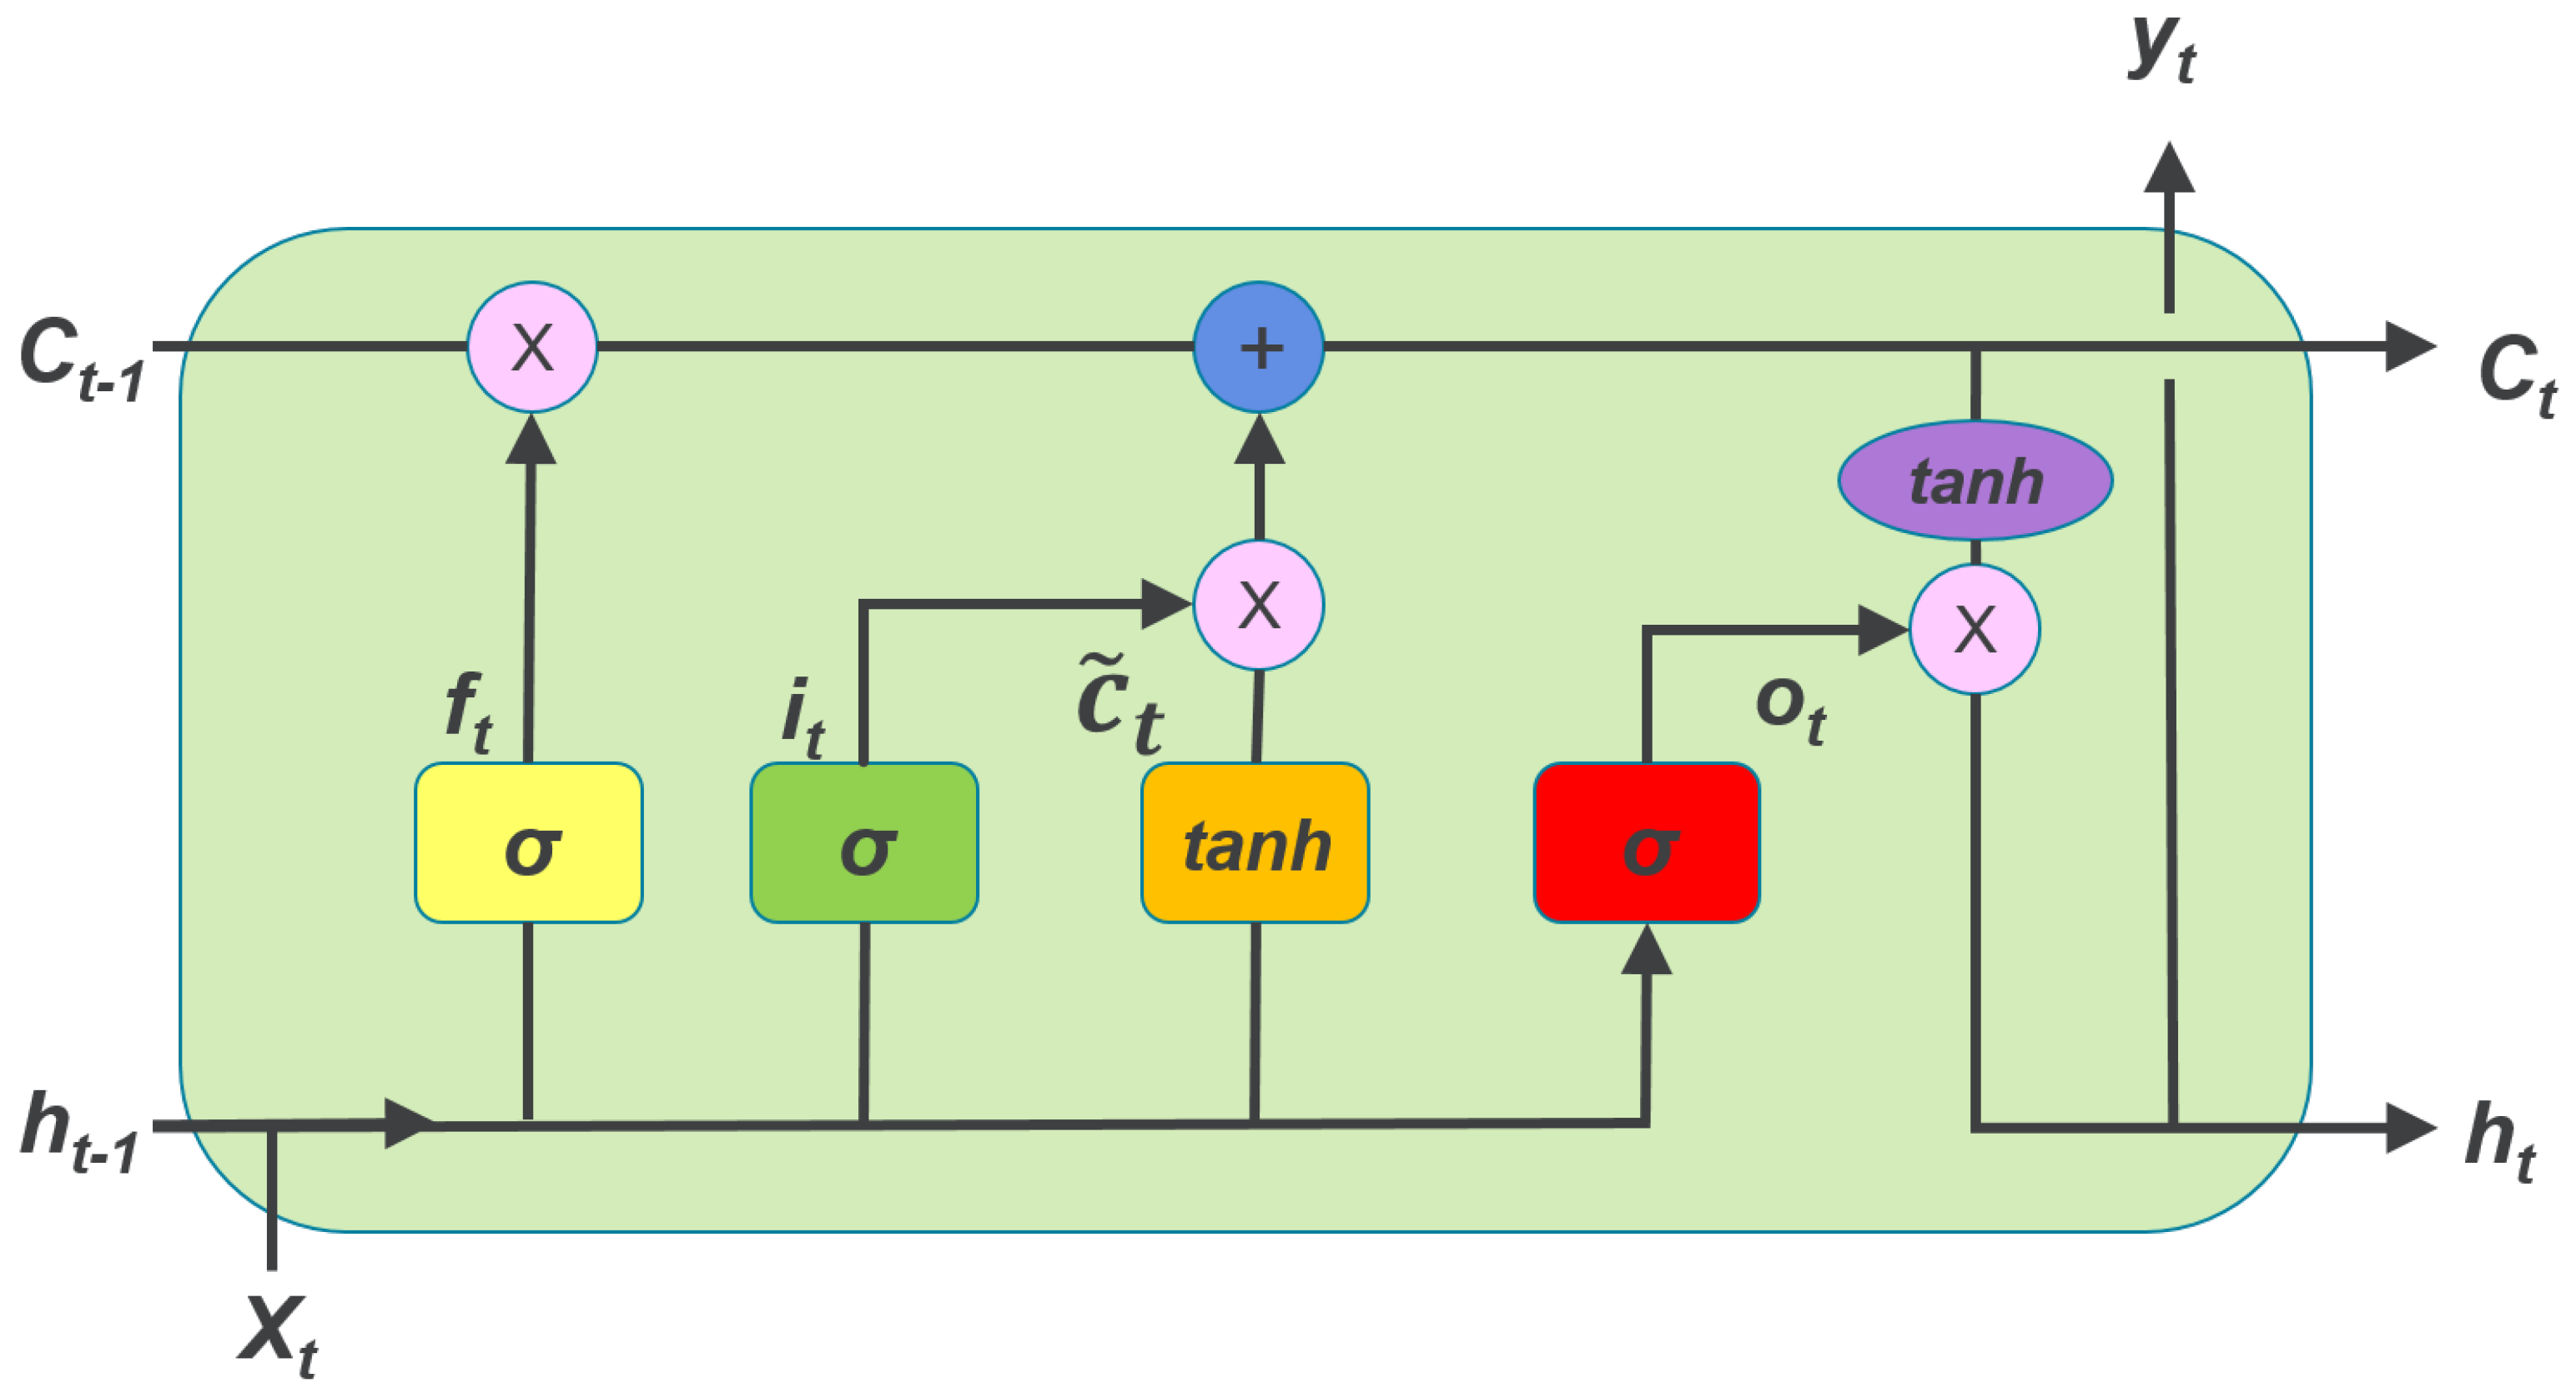
\includegraphics[width=0.7\columnwidth]{lstm} \\% Example image
    Figura 2. Long short-term memory
\end{center}

\section{Attention based models}

Our various  attention-based  models  are classifed
into two broad categories, global and local
. These classes differ in terms of whether the attention
is placed on all source positions or on only a few
source  positions.

Common to these two types of models is the fact
that at each time step $t$ in the decoding phase, both
approaches first take as input the hidden state $h_{t}$
at the top layer of a stacking LSTM. The goal is
then to derive a context vector $c_{t}$ that captures rel-evant source-side  information  to help predict  the current target word
$y_{t}$. While these models differ in how the context vector $c_{t}$
is derived, they share the same subsequent steps.

Specifically, given the target hidden state $h_{t}$
and the  source-side  context  vector $c_{t}$
,  we  employ  a simple concatenation  layer to combine the infor-mation 
from both vectors to produce an attentional hidden state as follows:

\begin{gather*}
  \widetilde{h_{t}} = tanh(W_{c}[c_{t},h_{t}])
\end{gather*}

The attentional vector $h_{t}$ is then fed through the
softmax  layer  to  produce  the  predictive  distribu-
tion formulated as:

\begin{gather*}
  p(y_{t}|y_{<t},x) = softmax(W_{s}\widetilde{h_{t}})
\end{gather*}

\subsection{Global attention}
The idea of a global attentional  model is to con-
sider all the hidden states of the encoder when de-
riving  the  context  vector $c_{t}$. In this  model  type,
a variable-length alignment vector $a_{t}$, whose size
equals the number of time steps on the source side,
is derived by comparing the current target hidden state
$h_{t}$ with each source hidden state $h_{s}$.

\begin{gather*}
  a_{t}(s) = align(h_{t},\bar{h_{s}})\\
           = \frac{ exp(score(h_{t},\bar{h_{s}})) }{ \sum_{s_{p}}exp(score(h_{t},h_{s})) }
\end{gather*}

\begin{center}
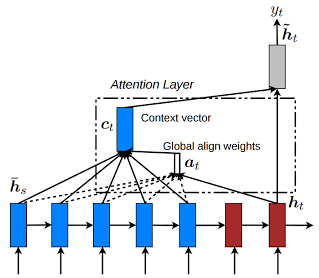
\includegraphics[width=0.7\columnwidth]{global} \\% Example image
    Figura 3. Global attentional model - at each time step t, the models infers a variable-length
    alignment weigth vector $a_{t}$ based on the current target state $h_{t}$ and all source states
    $\bar{h_{s}}$. A global context vector $c_{t}$ is then computed as the weighted average, according to $a_{t}$, over all the source states.
\end{center}

Here, score is referred as a \textit{content-based} function for which we consider three different alternatives:

\begin{gather*}
    score(h_{t},\bar{h_{s}}) =  \bar{h_{t}}^T \bar{h_{s}}       \\
    score(h_{t},\bar{h_{s}}) =  \bar{h_{t}}^T W_{a}\bar{h_{s}}   \\ 
    score(h_{t},\bar{h_{s}}) = \bar{v_{t}}^T Tanh( W_{a}[h_{t}:\bar{h_{s}}] )  \\
\end{gather*}

Besides alignment vector as weigths, the context vector $c_{t}$ is computed as the weight average over all the source
hidden states.


% \bar{q} 

\subsection{Local attention}
The global attention has a drawback that it has to
attend to all words on the source side for each tar-get word, which is expensive and can potentially
render it impractical to translate longer sequences, e.g.,  paragraphs  or  documents.   To  address  this
deficiency,  we propose  a local attentional  mech-anism that chooses to focus only on a small subset
of the source positions per target word. \\

This model takes inspiration from the tradeoff between the soft and hard attentional models proposed
by Xu et al.(2015) to tackle the image caption generation task. In their work, soft attention refers
to the global attention approach in which weights are placed "softly" over all patches in the source
image. The hard attention, on the order hand, selects on patch of the image to attend to a time.



\subsection{Input-feeding Approach}

In  our  proposed  global  and  local  approaches,
the attentional decisions are made independently,
which  is suboptimal.   Whereas,  in  standard  MT,
a coverage set  is  often  maintained  during  the
translation process to keep track of which source
words  have  been  translated.   Likewise,  in  atten-
tional NMTs, alignment decisions should be made
jointly  taking  into  account  past  alignment  infor-
mation.    To  address  that,  we  propose  an
input-feeding approach  in which attentional  vectors
$\bar{h_{t}}$ are concatenated with inputs at the next time
The  effects  of  hav-ing  such  connections  are  two-fold:  (a)  we  hope
to make the model fully aware of previous align-ment choices  and (b) we create a very deep net-
work spanning both horizontally and vertically.


\subsection{Figures}


\section{Experiments}
dsdsdsdsdsdsdsdsdsdsdsdsdsdsdsdsdsdsdsdsdsdsdsdsdsdsdsdsdsdsdsds
dsdsdsdsdsdsdsdsdsdsdsdsdsdsdsdsdsdsdsdsdsdsdsdsdsdsdsds
dsdsdsdsdsdsdsdsvdsdsdsddsdsdsdsdsdsdsdsdsdsdsds

\subsection{Training Details}
asdasdasd asdasdasd
asdasdasd
asdasdasd
asdasdasd
asdasdasd
asdasdasd

\subsection{English-Spanish Results}
asdasdasd asdasdasd
asdasdasd
asdasdasd
asdasdasd
asdasdasd
asdasdasd asdasdasd
asdasdasd
asdasdasd
asdasdasd
asdasdasd

\subsection{Spanish-English Results}
asdasdasd asdasdasd
asdasdasd
asdasdasd
asdasdasd
asdasdasd
asdasdasd asdasdasd
asdasdasd
asdasdasd
asdasdasd
asdasdasd

asdasdasd asdasdasd
asdasdasd
asdasdasd
asdasdasd
asdasdasd
asdasdasd asdasdasd
asdasdasd
asdasdasd
asdasdasd
asdasdasd

\section{Analysis}
dsdsdsdsdsdsdsdsdsdsdsdsdsdsdsdsdsdsdsdsdsdsdsdsdsdsdsdsdsdsdsds
dsdsdsdsdsdsdsdsdsdsdsdsdsdsdsdsdsdsdsdsdsdsdsdsdsdsdsds
dsdsdsdsdsdsdsdsvdsdsdsddsdsdsdsdsdsdsdsdsdsdsds

\subsection{Learning curves}

\subsection{Effects of Translations Long Sentences}

\subsection{Choices of attentional Architectures}

\subsection{Alignment Quality}

\subsection{Sample Translations}



\section{Conclusions}
This paragraph will end the body of this sample document.
Remember that you might still have Acknowledgments or
Appendices; brief samples of these
follow.  There is still the Bibliography to deal with; and
we will make a disclaimer about that here: with the exception
of the reference to the \LaTeX\ book, the citations in
this paper are to articles which have nothing to
do with the present subject and are used as
examples only.
%\end{document}  % This is where a 'short' article might terminate


% training details


\bibliographystyle{ACM-Reference-Format}
\bibliography{sample-bibliography} 

\end{document}
